\documentclass[a4paper, 12pt finnish]{article}
\usepackage[finnish]{babel}
\usepackage{graphicx}
\usepackage[utf8]{inputenc}
\usepackage[T1]{fontenc}

\title{Dokumentaatio \\ \large Tietokantasovellus}
\author{Joosua Laakso}
\date{\today}

\begin{document}
\maketitle

\section{Johdanto} 
\subsection{Työn aihe} Työn aiheena on työaikatietokanta. Sovellus on
suunniteltu erityisesti logistiikka-alan käyttöön. Tarkoituksena on, että
logistiikka-alalla työskentelevät autonkuljettajat voisivat paperisten
lomakkeiden täyttämisen sijaan syöttää tiedot työkeikkoihin käyttämästään
ajasta suoraan sovellukseen, jonka pitäisi huomattavasti vähentää 
työnantajan kirjanpitoasioihin käyttämää aikaa, koska tietoja ei enää
tarvitsisi kopioida käsin digitaaliseen muotoon paperisesta muodosta, vaan
ne olisi helposti saatavilla tietokannasta. Järjestelmään voi sisältyä
myös laskun automaattinen luonti, jonka avulla järjestelmään syötettyjen
tietojen perusteella, eli työntekijöiden syöttämien työaikatietojen ja 
työnantajan syöttämien tuntitaksatietojen, voisi luoda laskulomakkeen.

\subsection{Käytetyt tekniikat} Työ toteutetaan Helsingin yliopiston 
Users-palvelinta apuna käyttäen. Työssä käytetään Apache-palvelinsovellusta
sekä PHP-kieltä. Tietokannan hallintajärjestelmänä käytetään
Users-palvelimella paremmin tuettua PostgreSQL-järjestelmää.

\section{Yleiskuva järjestelmästä}
\subsection{Käyttäjäryhmät} Käyttäjät voidaan alustavasti eritellä kolmeen
yleisprofiiliin:
\paragraph{Jokamies} Jokamies viittaa kehen tahansa henkilöön, joka
vierailee tietokantasovelluksen web-sivuilla. Muut käyttäjäryhmät 
sisältyvät myös tähän joukkoon.
\paragraph{Johtaja} Johtoon kuuluvat henkilöt, joille työntekijät
työskentelevät, tai ketkä tahansa henkilöt joiden täytyy päästä käsiksi
työntekijöiden työaikatietoihin. Tähän ryhmään saattavat siis sisältyä myös
esimerkiksi kirjanpitäjät. Johto pääsee käsiksi kaikkiin jonkin
(työ)yhteisön tietoihin.
\paragraph{Työntekijä} Työntekijöihin kuuluvat käyttäjät, jotka syöttävät
työaikatietoja järjestelmään. Työntekijä kuuluu johonkin (työ)yhteisöön
ja kyseisen yhteisön johto näkee syötetyt työaikatiedot. Käyttäjä voi
kuulua sekä johtoon että työntekijöihin.

\subsection{Käyttötapaukset} Kullakin käyttäjäryhmällä on omia
käyttötapauksia. Ohessa on lueteltu näitä käyttötapauksia varustettuna
lyhyillä kuvauksilla. On kuitenkin huomioitava, että kaikkia
käyttötapauksia ei välttämättä kuitenkaan tueta lopullisessa versiossa,
vaan nämä ovat enemmän luonnoksenomaisia.

\paragraph{Jokamies:}
\subparagraph{Järjestelmään rekisteröityminen} Käyttäjän pitää pystyä
rekisteröitymään järjestelmän käyttäjäksi jotta voisi käyttää
järjestelmää. Rekisteröityminen tapahtuu rekisteröitymispalvelua käyttäen.

\paragraph{Johtaja:}
\subparagraph{Yhteisön rekisteröinti} Johtaja on aina johtaja jossain
yhteisössä. Jotta johtajalla olisi jokin yhteisö jota johtaa, täytyy
yhteisön rekisteröinnin olla mahdollista.
\subparagraph{Työaikatietojen katselu} Johtajalle täytyy olla mahdollista
seurata työntekijöiden syöttämiä työaikatietoja.
\subparagraph{Asiakkaan kirjaaminen} Johtajalle täytyy olla mahdollista
kirjata asiakkaan nimi muistiin (käytännössä usein jonkin yrityksen nimi).
Asiakkaaseen liittyy myös tuntitaksa, joka kirjataan myös järjestelmään. 
Asiakkaan poistamisen, sekä asiakkaan tietojen muokkaamisen ja jo 
kirjattujen asiakkaiden tietojen katselun täytyy myös olla tuettuna.
\subparagraph{Työntekijän kutsuminen yhteisöön} Johtajan täytyy pystyä
liittämään työntekijä siihen työyhteisöön järjestelmässä, johon 
työntekijä kuuluu. Työntekijän poistamisen yhteisöstä täytyy myös olla
mahdollista.
\subparagraph{Laskun luonti} Johtajalle olisi hyödyllistä, jos asiakkaan
tuntitaksatietojen sekä työntekijöiden lisäämien työaikatietojen pohjalta
voisi automaattisesti luoda laskun.

\paragraph{Työntekijä:}
\subparagraph{Yhteisöön liittyminen} Työntekijän täytyy pystyä liittyä
yhteisöön, johon johtaja on hänet kutsunut.
\subparagraph{Työaikatietojen syöttäminen} Työntekijän täytyy pystyä
lisäämään työaikatietoja järjestelmään. Työntekijän täytyy pystyä
valitsemaan kenelle asiakkaalle työ suoritettiin valikosta, joka sisältää
ne asiakkaat, joiden tiedot johtaja on syöttänyt järjestelmään. Tärkeää
on kuitenkin, että työntekijä ei pysty näkemään eri asiakkaiden
tuntitaksoja. Toisaalta täytyy kuitenkin olla mahdollista kirjata
järjestelmään jos aika käytettiin johonkin muuhun kun asiakkaalle
työskentelyyn, esimerkiksi auton viemiseen huoltoon tai jos asiakas oli
joku, jota ei löydy valikosta.

\subsection{Käyttötapauskaavio} Ohessa käyttötapaukset kuvattuna
graafisesti.

\begin{figure}[htbp]
    \centering
    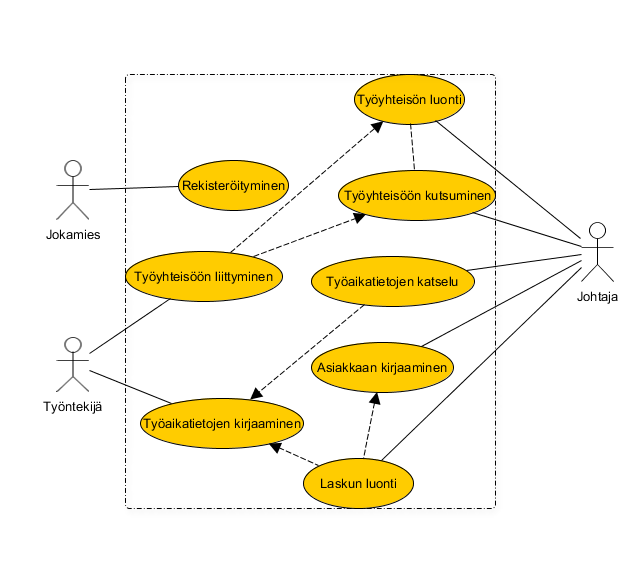
\includegraphics[width=1\textwidth]{graafi.png}
    \caption{\small Jos käyttötapaus on riippuvainen jostain toisesta
    käyttötapauksesta, se on merkitty katkoviivanuolella. Kaikki
käyttötapaukset ovat riippuvaisia rekisteröitymisestä, vaikka sitä
ei ole merkitty nuolella.}
\end{figure}
\newpage

\section{Järjestelmän tietosisältö}
\begin{figure}[h]
    \centering
    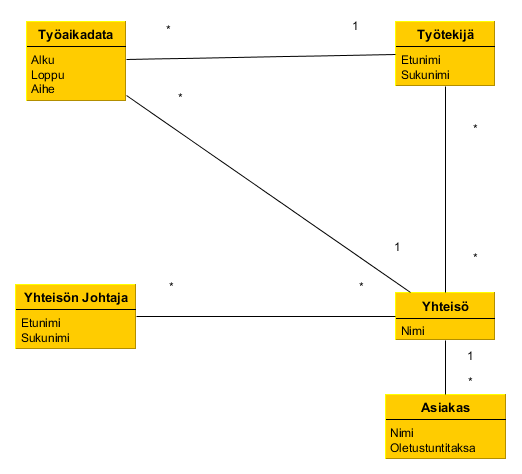
\includegraphics[width=0.8\textwidth]{maarittelykaavio.png}
    \caption{\small Alustava tietokohteita hahmotteleva kaavio.}
\end{figure} 

\subsection{Työaikadata}

\begin{center}
\begin{tabular}{| l | l | l |}
    \hline
    \emph{Attribuutti} & \emph{Tyyppi} & \emph{Kuvaus} \\ \hline
    Alku & timestamp & Työtapahtuman alkamisaika \\ \hline
    Loppu & timestamp & Työtapahtuman loppumisaika \\ \hline
    Aihe & string & Tekstikuvaus työtapahtumasta \\ \hline
\end{tabular}
\end{center}

Työaikadataan saattaa liittyä yksi asiakas. Työaikadataan liittyy yksi
työntekijä. Työaikadata liittyy johonkin yhteisöön.

\subsection{Työntekijä}
\begin{center}
\begin{tabular}{| l | l | l |}
    \hline
    \emph{Attribuutti} & \emph{Tyyppi} & \emph{Kuvaus} \\ \hline
    Etunimi & string & Työntekijän etunimi \\ \hline
    Sukunimi & string & Työntekijän sukunimi \\ \hline
\end{tabular}
\end{center}

Työntekijä voi kuulua moneen yhteisöön ja työntekijään voi liittyä
monta työaikadatapistettä.

\subsection{Yhteisö}
\begin{center}
\begin{tabular}{| l | l | l |}
    \hline
    \emph{Attribuutti} & \emph{Tyyppi} & \emph{Kuvaus} \\ \hline
    Nimi & string & Yhteisön nimi \\ \hline
\end{tabular}
\end{center}

Yhteisöön voi kuulua useita asiakkaita. Yhteisöllä voi olla useita
jäseniä, joista useat voivat olla johtajia. Yhteisöön voi liittyä
useita eri työaikadatapisteitä, joita yhteisön jäsenet ovat kirjanneet
järjestelmään. Yhteisö viittaa työyhteisöön joka käytännössä on usein
jokin kuljetusyritys. Tietokohteen nimi ei kuitenkaan ole yritys siksi,
koska esimerkiksi samalla yrityksellä voi olla palvelussa useita eri 
yhteisöjä.

\subsection{Yhteisön johtaja}
Johtaja on käyttäjä, jolla on yhteisönjohtamisetuoikeudet. Johtaja pääsee
käsiksi kaikkiin yhteisöön liittyviin tietoihin, joihin lukeutuvat
esimerkiksi asiakkaiden oletustuntitaksat sekä yhteisön jäsenten 
kirjaamat tunnit. Käyttäjä voi olla usean eri yhteisön johtaja.

\subsection{Asiakas}
\begin{center}
\begin{tabular}{| l | l | l |}
    \hline
    \emph{Attribuutti} & \emph{Tyyppi} & \emph{Kuvaus} \\ \hline
    Nimi & string & Asiakkaan nimi, käytännössä jonkin yrityksen nimi \\
    \hline
    Oletustuntitaksa & decimal & Asiakkaan oletustuntitaksa euroissa \\
    \hline
\end{tabular}
\end{center}

Asiakas kuuluu vain yhteen yhteisöön, siitä huolimatta että käytännössä
sama asiakas saattaa tilata palveluja usealta eri työyhteisöltä. Tämä
siksi koska tuntitaksat saattavat kuitenkin vaihdella eri työyhteisöillä,
joten on helpompaa toteuttaa asiakkaan ja yhteisön yhteys näin. 
Asiakas voi liittyä työaikadataan, mutta se tapahtuu välillisesti
yhteisön kautta.

\newpage
\section{Relaatiotietokantakaavio}
\begin{figure}[htbp]
    \centering
    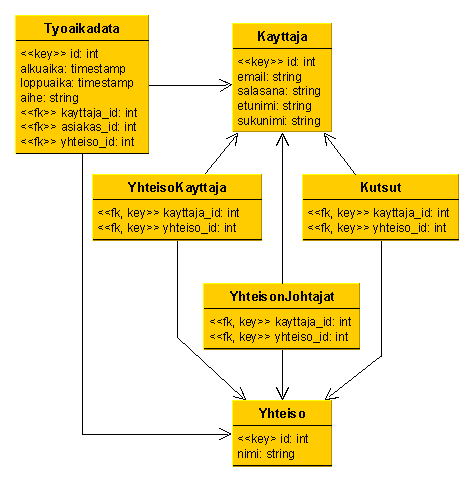
\includegraphics[width=1\textwidth]{relaatiokaavio.png}
    \caption{\small Alustava kaavio jossa on graafisesti hahmoteltuna
    relaatiotietokannan taulut ja niiden yhteydet}
\end{figure}

\section{Käyttöliittymä}
\subsection{Käyttöliittymäluonnokset}
Ohessa muutama luonnos käyttöliittymästä.
\begin{figure}[htbp]
    \centering
    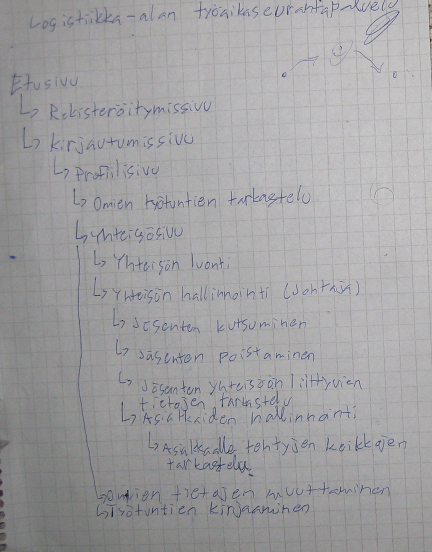
\includegraphics[width=0.8\textwidth]{sivukartta.png}
    \caption{\small Navigointia havainnollistava sivukartta}
\end{figure}
\begin{figure}[htbp]
    \centering
    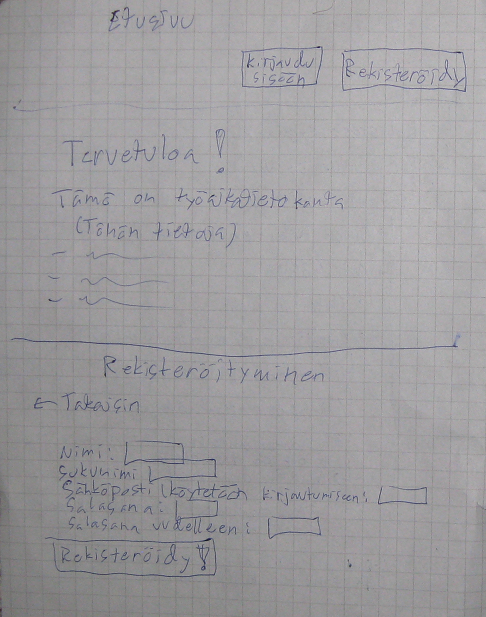
\includegraphics[width=0.8\textwidth]{etusivu.png}
    \caption{\small Etusivu ja rekisteröityminen}
\end{figure}
\begin{figure}[htbp]
    \centering
    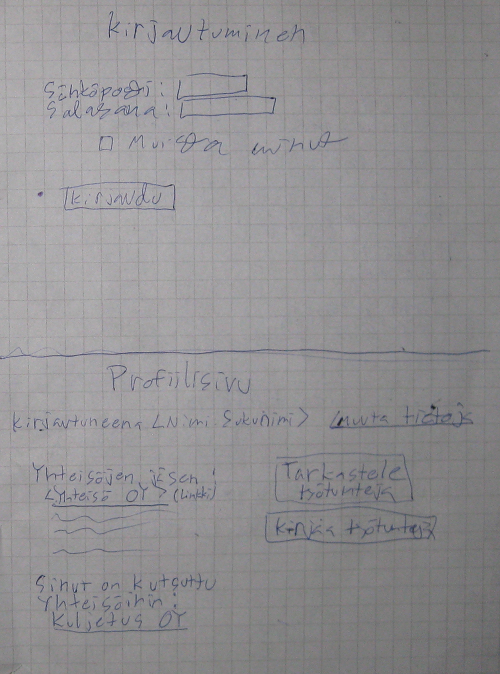
\includegraphics[width=0.8\textwidth]{kirjautuminen.png}
    \caption{\small Kirjautuminen ja profiilisivu}
\end{figure}
\begin{figure}[htbp]
    \centering
    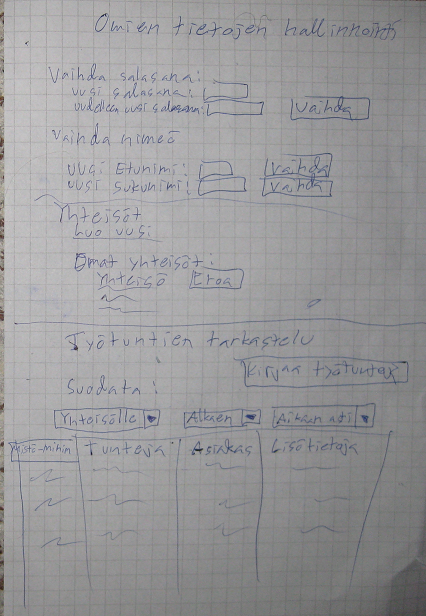
\includegraphics[width=0.8\textwidth]{omattiedot.png}
    \caption{\small Käyttäjän tietojen hallinnointi ja työtuntien
    tarkastelu}
\end{figure}
\begin{figure}[htbp]
    \centering
    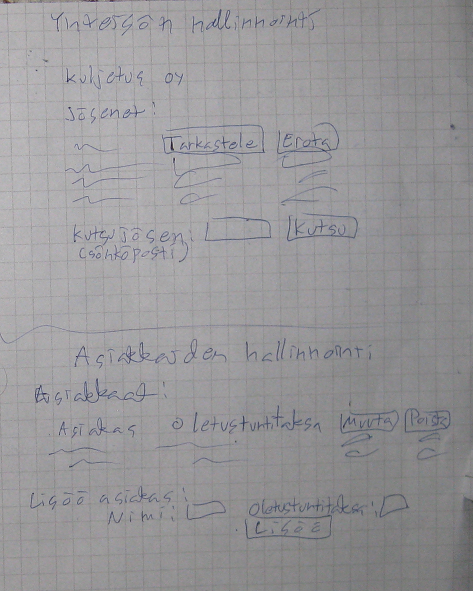
\includegraphics[width=0.8\textwidth]{yhthallinnointi.png}
    \caption{\small Yhteisön hallinnointi ja asiakkaiden tietojen
    hallinnointi}
\end{figure}
\begin{figure}[htbp]
    \centering
    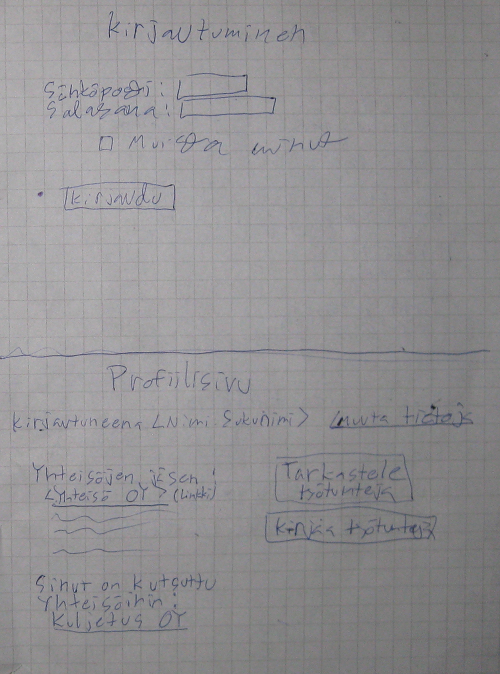
\includegraphics[width=0.8\textwidth]{kirjaaminen.png}
    \caption{\small Työtuntien kirjaaminen ja yhteisön sivut}
\end{figure}

\section{Järjestelmän yleisrakenne} Järjestelmä noudattaa MVC-mallia,
jossa ohjelmiston eri tehtävät on jaettu omiin kerroksittaisiin
kokonaisuuksiin. Kansiost views löytyy näkymät, jotka määrittelevät
käyttöliittymän graafisen ilmeen. Kontrollerit sijaitsevat juuressa ja
niiden tehtävä on ottaa vastaan käyttäjän antamia käskyjä sekä antaa
näkymille tieto siitä, millaista dataa käyttäjälle näytetään. Kansiossa
libs on erilaisia kirjastoja ja kontrollerien toiminnallisuutta jatkavia
tiedostoja. Näistä kirjastoista tärkein lienee commons.php, jossa on
erilaisia yleiskäyttöisiä funktioita. Libs-kansiossa on alakansio models,
jossa sijaitsevat mallit, joiden tehtävä on tarjota käyttöliittymä 
projektissa käytettävään PostgreSQL-tietokantaan. Kaikki tiedostojen ja
kansioiden nimet on kirjoitettu pienillä alkukirjaimilla.

\section{Käyttöliittymä ja järjestelmän komponentit} Ohessa on esitettynä
suppea kaavio joka kuvaa, miten sivustolla navigointi tapahtuu.
\begin{figure}[htbp]
    \centering
    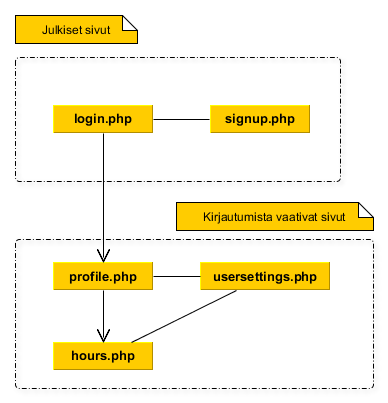
\includegraphics[width=0.8\textwidth]{kayttoliittymakaavio.png}
    \caption{\small Sivustolla navigointi}
\end{figure}

\section{Asennustiedot} Sovelluksen voi asentaa siirtämällä
sovelluksen tiedostot sellaiseen hakemistoon, joka näkyy
verkkoon. Tietokantataulut voi pystyttää suunnistamalla
komentotulkilla 'sql'-kansioon ja suorittamalla käskyn
'psql < create-tables.sql'. Tietokantataulut voi ajaa
alas käskyllä 'psql < drop-tables.sql'.

\section{Käyttöohje} Sovellusta voi käyttää osoitteessa
'jola.users.cs.helsinki.fi/login.php'.
Testikäyttäjätunnus on 'test@testing.com' ja
testisalasana testikäyttäjätunnukselle on 'salasana'.
\end{document}
